\documentclass[12pt]{article}

\usepackage{fullpage}
\usepackage{multicol,multirow}
\usepackage{tabularx}
\usepackage{ulem}
\usepackage{graphicx}%Вставка картинок правильная
\usepackage{float}%"Плавающие" картинки
\usepackage{wrapfig}%Обтекание фигур (таблиц, картинок и прочего)
\usepackage[utf8]{inputenc}
\usepackage[russian]{babel}

% Оригиналный шаблон: http://k806.ru/dalabs/da-report-template-2012.tex

\begin{document}

\section*{Курсовой проект по курсу дискрeтного анализа: Текстовый поиск}

Выполнил студент группы 08-307 МАИ \textit{Дегтярев Денис Андреевич}.

\subsection*{Условие}

Реализуйте систему для поиска статей по заданным словам.  
\textbf{Формат запуска в режиме индексации}
\begin{verbatim}
./prog index --input <input file> \
                --output <index file>
\end{verbatim}

\begin{itemize}
    \item \texttt{--input}: входной файл со статьями
    \item \texttt{--output}: выходной файл с индексом
\end{itemize}

\textbf{Формат запуска в режиме поиска}
\begin{verbatim}
./prog search --index <index file> \
                --input <input file> \
                --output <output file> \
                [--full-output]
\end{verbatim}

\begin{itemize}
    \item \texttt{--index}: входной файл с индексом
    \item \texttt{--input}: входной файл с запросами
    \item \texttt{--output}: выходной файл с ответами на запросы
    \item \texttt{--full-output}: переключение формата выходного файла на подробный
\end{itemize}

\subsection*{Формат ввода}

\textbf{Формат файлов для индексации:}
\begin{verbatim}
<doc id="12" url="https://en.wikipedia.org/wiki?curid=12" title="Anarchism">
<текст статьи>
</doc>
<doc id="25" url="https://en.wikipedia.org/wiki?curid=25" title="Autism">
<текст статьи>
</doc>
\end{verbatim}
\textbf{Формат файла с запросами:}
\begin{verbatim}
<word 1>
<word 1> & <word 2>
<word 1> | <word 2>
~<word 1>
~(<word 1> & <word 2> & <word 3>) | (<word 4> & (<word 5> | ~<word 6>))
\end{verbatim}

\subsection*{Формат вывода}

\textbf{Формат выходного файла в режиме индеексации:}
\begin{verbatim}
Бинарный файл, в котором хранится unordered_map и вектор названий статей
\end{verbatim}
\textbf{Формат выходного файла в режиме поиска:}
\begin{verbatim}
Если опция --full-output не указана: на каждый запрос в отдельной строке выводится количество
документов подпадающих под запрос.
Если опция --full-output указана: на каждый запрос выводится отдельная строка, с количеством
документов подпадающих под запрос, а затем названия всех документов подпадающих под запрос по
одному названию в строке.
\end{verbatim}

\subsection*{Метод решения}

\textbf{Индексация:}
\begin{itemize}
    \item Создаем хэш таблицу:
    \begin{itemize}
        \item[-] ключ: слово
        \item[-] значение: название файла, где хранится очередь из номеров на каждое слово
    \end{itemize}
    \item Заполняем файлы, где хранится очередь из номеров на каждое слово
    \item Создаем массив:
    \begin{itemize}
        \item[-] индекс: номер текста
        \item[-] значение: название текста
    \end{itemize}
    \item Сохраняем хэш таблицу
    \item Сохраняем массив
\end{itemize}
\textbf{Поиск:}
\begin{itemize}
    \item Загружаем хэш таблицу и в случае флага --full-output - массив
    \item Преобразуем операции над множествами в польскую запись
    \item Выполняем операции над статьями, в которых содержатся слова в запросах:
    \begin{itemize}
        \item[-] преобразуем файл соответствующего слова, где хранятся индексы статей, в очередь из этих индексов
        \item[-] выполняем операции над очередями по ходу поступления в польской записи
    \end{itemize}
    \item Выводим результат:
    \begin{itemize}
        \item[-] без флага --full-output: выводим размер очереди
        \item[-] с флагом --full-output: выводим размер очереди и в каждой строке название соответствующего индексу, находящемуся в очереди, статьи
    \end{itemize}
\end{itemize}

\subsection*{Описание программы}
\begin{verbatim}
src
|- main.cpp: получает на вход все входные данные и обрабатывает их
lib
|- function.hpp: содержит вспомогательные функции
|- index.hpp: содержит функции, превращающие текст в формат, удобный для хранения
   и дальнейшего использования для поиска
|- library.hpp: содержит нужные для программы библиотеки
|- load.hpp: содержит функции, превращающиеся файлы в нужный формат для дальнейших
   вычислений
|- operator.hpp: содержит функции для операций пересечения, объединения,
   логического нет
|- parser.hpp: содержит парсеры, обрабатывающие аргументы при запуске программы
   и запросы при поиске
|- save.hpp: содержит функции, преобразующие слова и статьи, в которых они содержатся
   в удобный для хранения и запуска формат
|- search.hpp: содержит функции, преобразующие запросы в постфиксный вид и производящие
   вычисления операций над множествами
\end{verbatim}

\subsection*{Тест производительности}

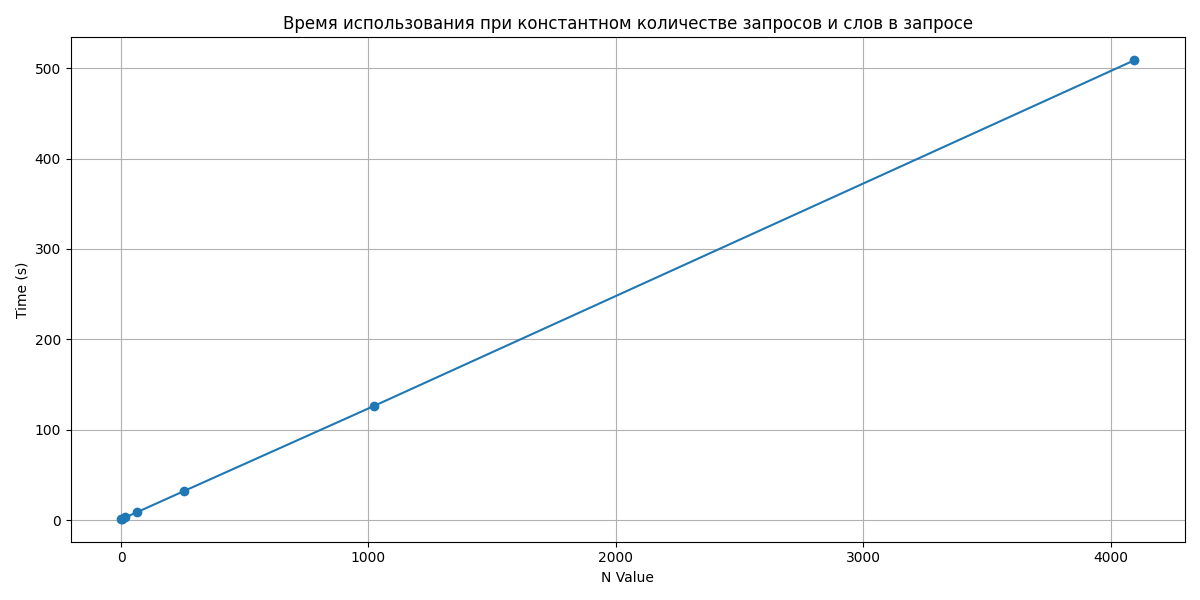
\includegraphics[width=7in]{Figure_1.png}

\subsection*{Особенности программы}

\begin{itemize}
    \item Все операции вставки выполняются за \( O(1) \).
    \item Операции пересечения и объединения в режиме поиска суммарно выполняются за \( O\left(\sum_{i=1}^{k} \text{queue}_i.\text{size}()\right) \), где \( k \) - количество знаков & или | в запросе. То есть, при одном слове в строке поиска, поиск будет выполняться за \( O(1) \).
    \item Операция логического "нет" выполняется за \( O(n) \), где \( n \) - количество всевозможных статей.
    \item Никакой нагрузки на оперативную память, даже при огромном числе слов за счет хранения нужной информации на жестком диске.
    \item Все операции при поиске линейны, что обеспечивает высокую скорость работы.
\end{itemize}

\subsection*{Выводы}

В процессе реализации инвертированного индекса и алгоритма поиска по текстам для написания курсового проекта по предмету «Дискретный анализ» я достиг нескольких важных целей и узнал много нового:

\begin{enumerate}
    \item \textbf{Понимание инвертированных индексов}: Я получил глубокое понимание того, как работают инвертированные индексы, которые являются основой многих систем полнотекстового поиска. Это знание может быть применено в разработке поисковых систем и в обработке больших объёмов текстовых данных.
    \item \textbf{Работа с хэш-таблицами}: Я использовал \texttt{unordered\_map} для создания индекса, что помогло мне практически применить знания о хэш-таблицах, включая их эффективность и способы применения в реальных задачах.
    \item \textbf{Алгоритмическое мышление}: Решение задачи требовало алгоритмического подхода, в частности, для определения пересечения наборов текстов. Это укрепило мои навыки в области алгоритмов и структур данных.
    \item \textbf{Работа со строками и текстовыми данными}: Я практиковался в обработке и анализе строк, что полезно во многих областях программирования, от разработки программного обеспечения до анализа данных.
    \item \textbf{Проблемы масштабируемости и оптимизации}: Я столкнулся с вопросами масштабируемости и оптимизации при обработке большого количества текстов и запросов, что представляет собой важный аспект в разработке производительных приложений.
    \item \textbf{Умение решать практические задачи}: Я успешно применил теоретические знания для решения практической задачи, что является важным навыком в любой инженерной дисциплине.
\end{enumerate}

Таким образом, выполнение этой работы не только помогло мне развить технические навыки в области компьютерных наук, но и дало ценный опыт в решении реальных задач, который может быть применен в будущих проектах.

\end{document}
